\section{Free Carrier Statistics}
In order to draw conclusions about material properties by analyzing
the temperature dependence of the charge carrier density,
free carrier statistics and especially the influence of doping shall be
discussed.
\subsection{Charge Carrier Density}
The number of electrons per volume in the conduction band $n$ is
determined by the following expression:
\begin{equation}
	n=\int _{E_{\mathrm{C}}}^{\infty} D_{\mathrm{e}}(E)
	f_{\mathrm{e}}(E)\, \mathrm{d}E.
	\label{eq:n_int}
\end{equation}
In this equation, $E_{\mathrm{C}}$ represents the minimum energy level of
the conduction band. The function $D_{\mathrm{e}}(E)$ describes
the density of electronic states at a given energy $E$, while
$f_{\mathrm{e}}(E)$ is the statistical distribution function.
For electrons, this function is the Fermi-Dirac distribution that can be
defined with $E_\mathrm{f}$ as the Fermi-energy, $\mathrm{k}$ as the
Boltzmann constant and $T$ as temperature:
\begin{equation}
	f_{\mathrm{e}}(E)
	=\frac{1}{\exp((E-E_{\mathrm{F}})/(\mathrm{k}T))+1}.
\end{equation}
In order to solve the integral in \cref{eq:n_int}, one needs a functional
expression for the density of states.
A suitable approximation that utilizes the effective electron mass
$m^*_\mathrm{e}$ are
parabolic band edges which originates from the free-electron gas:
\begin{equation}
	D(E)=\frac{1}{2\pi^2}
	\left( \frac{2m^*_\mathrm{e}}{\hbar^2} \right)^{3 / 2} \sqrt{E}.
	\label{eq:para_band_edges}
\end{equation}
If one substitutes \cref{eq:para_band_edges} into \cref{eq:n_int} and uses
the transformations $\eta=E_\mathrm{F}-E_\mathrm{C}$,
$x = (E-E_\mathrm{C}) / (\mathrm{k} T)$, the integral can be brought into
the following form:
\begin{align}
	n            & = N_\mathrm{c} \frac{2}{\sqrt{\pi}}
	\int_{0}^{\infty} \frac{\sqrt{ x }}{1+\exp(x-\eta / (\mathrm{k}T))} \,
	\mathrm{d}x \label{eq:n_int_2},                                        \\
	N_\mathrm{c} & = 2 \left( \frac{2 \pi m^*_\mathrm{e} \mathrm{k}T}{h^2}
	\right)^{3 / 2}.
\end{align}
\Cref{eq:n_int_2} represesnts a form of the Fermi-Dirac integral
$F_{1 /2}(\eta  / (\mathrm{k}T))$.
For $0 \gg \eta$,
this function can be approximated by $F_{1 /2}(\eta  / (\mathrm{k}T))
	\simeq \exp(\eta /(\mathrm{k}T))$.
Semiconductors that fulfill this requirement all called degenerate.
With that approximation, the free carrier density can be expressed as
a function of Fermi-energy:
\begin{equation}
	n	= { N_{\mathrm{C}} }\exp\left( \frac{E_{\mathrm{F}}
		-E_{\mathrm{C}}}{\mathrm{k_B}T} \right).
	\label{eq:n}
\end{equation}
The same procedure can be applied analogous for holes instead of
electrons.
One finds with similar assumptions:
\begin{align}
	p            & = N_\mathrm{V} \exp
	\left( - \frac{E_{\mathrm{F}}-E_{\mathrm{V}}}{\mathrm{k}T} \right)^{3 / 2}
	\label{eq:p},                                        \\
	N_\mathrm{V} & = 2 \left( \frac{2 \pi m^*_\mathrm{h}
		\mathrm{k}T}{h^2} \right).
\end{align}

\subsection{Intrinsic Conduction}
For an ideally pure semiconductor, only valence-band electrons
can exite into the conduction band.
This leads to the following charge neutrality condition:
\begin{equation}
	n = p.
\end{equation}
With this additional constraint, a formula for the free
carrier concentration can be found that only depends on the
band gap $E_\mathrm{g} = E_\mathrm{C} - E_\mathrm{V}$ by
substituting \cref{eq:n} and \cref{eq:p}
into the root:
\begin{align}
	p & = n = \sqrt{n^2} = \sqrt{n \cdot p} \notag \\
	  & =\sqrt{ N_{\mathrm{V}}N_{\mathrm{C}} }
	\exp\left( -\frac{E_{\mathrm{g}}}{2\mathrm{k}T} \right).
\end{align}

\subsection{Donors and Acceptors}
\begin{figure*}
	\centering
	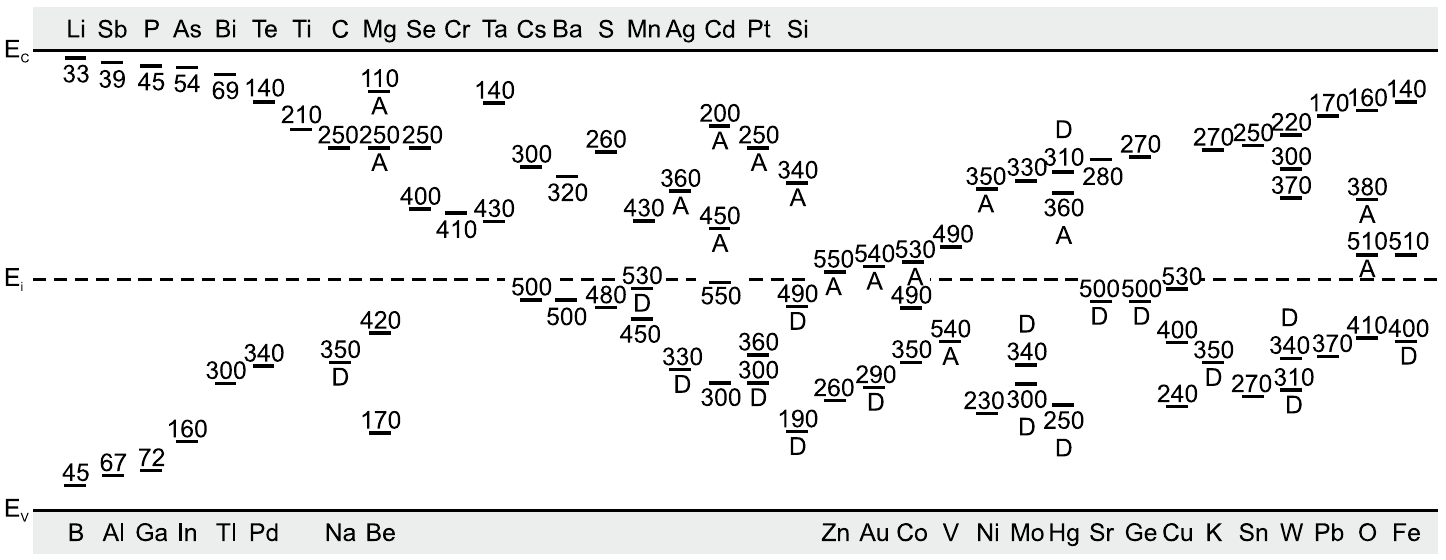
\includegraphics[width=0.6\linewidth]{../assets/energy_level.png}
	\caption{Energetic position of various donors and acceptors
		for silicon. \imcite{grundmann}}
	\label{fig:energy_level}
\end{figure*}

The conductivity of a semiconductor can be altered using
point defects.
This process is called doping.
If the conductivity is determined by holes, the material is
called p-type.
If the conductivity is determined by electrons, the material
is called n-type.

\paragraph{Donors} are point defect atoms that are incorporated into the crystal
lattice and dispose an additional electron after satisfying all
lattice bonds.
For group-$\mathrm{IV}$ semiconductors, group-$\mathrm{V}$ elements
are donors.
This extra electron is bound to the atom via Coulomb interaction,
which is a result of the higher charge of the donor's core.
The energy level of this electron can be estimated by assuming
energetically rescaled hydrogen orbitals.
This rescaling originates from the effective electron mass and
the screening of the coulomb interaction by the dielectric constant
of the material.
The absolute energetic position of the bound electron is
$E_{\mathrm{D}}=E_{\mathrm{C}}-E_{\mathrm{D}}^{b}$ with
\begin{equation}
	E_{\mathrm{D}}^{b}=
	\frac{1}{\epsilon_{\mathrm{r}}^{2}}
	\frac{m_{\mathrm{e}}^{*} e^{4}}{2(4\pi\epsilon_{0}\hbar)^{2}}.
\end{equation}
Energetic positions of various donors are displayed in
\cref{fig:energy_level}.
Similar to intrinsic conduction, the additional electrons have a
finite probability to shift into the conduction band
(they donate an electron) and
can therefore be used for n-type doping.
The probability for an electron to occupy the bound state $f^0$
(where $0$ indicates that the donor is neutral) can be expressed
by the Fermi-Dirac distribution.
The probability for an electron to not occupy the bound state $f^+$
(where $+$ indicates that the donor is ionized) can also be
determined:
\begin{align}
	f_{0} & =\frac{1}{1+\frac{g_{+}}{g_{0}}\exp\left(
	\frac{E_{\mathrm{D}}-E_{\mathrm{F}}}{\mathrm{k}T}\right)},  \\
	\label{eq:fplus}
	f_{+} & =(1-f_{0})=\frac{1}{1+\frac{g_{0}}{g_{+}}\exp\left(
		\frac{E_{\mathrm{F}}-E_{\mathrm{D}}}{\mathrm{k}T} \right)}.
\end{align}
Note that the degeneracy of the states impact the distribution.
A neutral donor has a degeneracy of $g^0=2$, since the bound
electron can take two spin states, the degeneracy of the
ionized donor is simply $g^+=1$.

Either the electron occupies the bound state or it shifts into the
conduction band.
Let $N_\mathrm{d}$ be the donor concentration, $N_\mathrm{d}^0$ the
number of neutral donors and $N_\mathrm{d}^+$ the number of ionized donors.
One finds the following relations:
\begin{align}
	N_{\mathrm{D}}     & =N_{\mathrm{D}}^{+}+N_{\mathrm{D}}^{0},        \\
	N_{\mathrm{D}}^{0} & =N_{\mathrm{D}}f_0                             \\
	\label{eq:ndplus}
	N_{\mathrm{D}}^{+} & =N_{\mathrm{D}}(1-f_{0}) =N_{\mathrm{D}}f_{+}.
\end{align}

\paragraph{Acceptors} are point defect atoms that are incorporated
into the crystal
lattice and lack one binding electron.
They are able to borrow (accept) an electron from the valence band.
For group-$\mathrm{IV}$ semiconductor, elements from group-$\mathrm{III}$
can be used as acceptors.
The energetic considerations are similar to those of donors.
The energy level of an electron that is bound to the acceptor can be
expressed
$E_{\mathrm{A}}=E_{\mathrm{V}}+E_{\mathrm{A}}^{b}$,
where $E_\mathrm{A}^b$ can be represented by rescaled
hydrogen orbitals.

These levels are also displayed in \cref{fig:energy_level}.
The total number of acceptors $N_\mathrm{A}$ can be separated into
the number of ionized acceptors $N_\mathrm{A}^-$ and neutral
acceptors $N_\mathrm{A}^0$, such that the relation
$N_{\mathrm{A}}=N_{\mathrm{A}}^{0}+N_{\mathrm{A}}^{-}$ holds.
Again the probability of finding an electron bound to an acceptor $f$ is
equal to the probability of a hole shifted from the acceptor to the
valence band and can be modelled by a Fermi-distribution:
\begin{equation}
	f = \frac{1}{1+\hat{g}_{\mathrm{A}}\exp\left( -
	\frac{E_{\mathrm{F}}-E_{\mathrm{A}}}{\mathrm{k}T} \right)}.
\end{equation}
In this case, the ratio of the acceptor state degeneracies
$\hat{g}_\mathrm{A}$ are nontrivial and need to be considered in detail.

\subsection{Charge Neutrality Condition}
The most general charge neutrality condition can be expressed as:
\begin{equation}
	n = p -\sum_i N_{\mathrm{A}i}^- + \sum_j N_{\mathrm{D}j}^+.
\end{equation}
This can be used to get an implicit functional dependence $f(n,T)$.
A simple example is a material that is doped by only one donator material.
If one uses \cref{eq:ndplus} and additionally assume sufficient low
temperatures, intrinsic conduction can be neglected and the charge
neutrality condition is reduced to $n = N_\mathrm{D}^+=N_\mathrm{D} f_+$.
By substituting \cref{eq:n} and \cref{eq:fplus} and rearranging the
equation, one obtains:
\begin{align}
	\notag
	n     & =\frac{N_{\mathrm{D}}}{1+\hat{g}
		\exp\left( \frac{E_{\mathrm{F}}-E_{\mathrm{C}}}{\mathrm{k}T} \right)
	\exp\left( \frac{E_{\mathrm{C}}-E_{\mathrm{D}}}{\mathrm{k}T} \right)}                   \\
	\notag
	      & =\frac{N_{\mathrm{D}}}{1+ \hat{g}n /N_{\mathrm{C}}\cdot
	\exp\left( \frac{E_{\mathrm{C}}-E_{\mathrm{D}}}{\mathrm{k}T} \right)} \label{eq:n_quad} \\
	      & =\frac{N_{\mathrm{D}}}{1+n / n_{1}}                                             \\
	n_{1} & =	\frac{N_{\mathrm{C}}}{\hat{g}}
	\exp\left( -\frac{E_{\mathrm{D}}^{b}}{\mathrm{k}T} \right)
\end{align}
\Cref{eq:n_quad} is a quadratic equation in terms of $n$ and thus
analytically solvable.
This leads to an explicit temperature dependence that can be approximated
for low and high temperature. 
\begin{equation}
	\label{eq:n_T}
	n=\frac{2N_{\mathrm{D}}}
	{1+\left( 1+4\hat{g} \frac{N_{\mathrm{D}}}{N_{\mathrm{C}}}
		\exp\left( \frac{E_{\mathrm{D}}^{b}}{\mathrm{k}T} \right) \right)^{1/2}}.
\end{equation}
\begin{align}
	\label{eq:n_T_approx_low}
	n & \simeq \sqrt{ \frac{N_{\mathrm{D}}N_{\mathrm{C}}}{\hat{g}} }
	\exp\left( \frac{-E_{\mathrm{D}}^{b}}{2 \mathrm{k}T} \right) & \mathrm{k}T\ll E_{\mathrm{D}}^{b} \\
	n & \simeq N_{\mathrm{D}} & \mathrm{k}T\gg E_{\mathrm{D}}^{b}
\end{align}

\begin{figure}
	\centering
	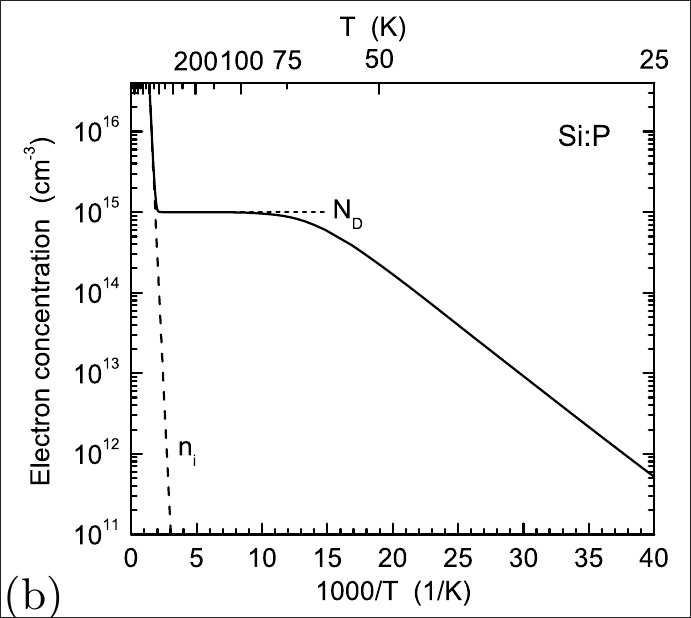
\includegraphics[width=0.6\linewidth]{../assets/charge_carrier_density_temperature.png}
	\caption{Charge carrier density as a function of temperature for 
	silicon doped with phosphor. \imcite{grundmann}}
	\label{fig:carrier_temperature}
\end{figure}
The function $n(T)$ is visualized in \cref{fig:carrier_temperature}.
Note that intrinsic conduction cannot be neglected for sufficient high
temperatures.
\imcite{grundmann}